\documentclass[11pt]{article}
\usepackage[scaled=0.92]{helvet}
\usepackage{geometry}
\geometry{letterpaper,tmargin=1in,bmargin=1in,lmargin=1in,rmargin=1in}
\usepackage[parfill]{parskip} % Activate to begin paragraphs with an empty line rather than an indent %\usepackage{graphicx}
\usepackage{amsmath,amssymb, mathrsfs, dsfont}
\usepackage{tabularx}
\usepackage[font=footnotesize,labelfont=bf]{caption}
\usepackage{graphicx}
\usepackage{xcolor}
%\usepackage[linkbordercolor ={1 1 1} ]{hyperref}
%\usepackage[sf]{titlesec}
\usepackage{natbib}
\usepackage{../../Tianpei_Report}


\begin{document}
\title{Self-study: Variational Wasserstein Problems}
\author{Tianpei Xie}
\date{ Aug. 19th., 2022 }
\maketitle
\tableofcontents
\newpage
\section{Previous lessons}
\begin{itemize}
\item Recall the definition of Wasserstein distance between two measures $\alpha, \beta\in \cM(\cX)$, where $\cM(\cX)$ is the space of Radon measure on $\cX$: 
\begin{definition}
We suppose $\cX = \cY$ and that for some $p \ge 1$, $c(x,y)= d(x,y)^p$, where $d$ is a distance on $\cX$, i.e. 
\begin{enumerate}
\item $d(x, y) = d(y, x)$ for all $x, y\in \cX$; 
\item $d(x, y)  = 0$ iff  $x=y$;
\item $d(x, y) \le d(x, z) + d(z, y)$, for all $x, y, z \in \cX$
\end{enumerate}
Then the \emph{\textbf{$p$-Wasserstein distance}} between $\alpha, \beta \in \cM_{+}^{1}(\cX)$ on $\cX$ is defined by $\cW_{p}(\alpha, \beta) := \cL_{d^{p}}(\alpha, \beta)^{\frac{1}{p}}$, where $\cX = \cY$ and 
\begin{align*}
 \cL_{d^{p}}(\alpha, \beta) := \min_{\pi \in \cM_{+}^{1}(\cX \times \cY)}& \int_{\cX \times \cY} d^{p}(x, y) d \pi(x, y)  \\
\text{s.t. }& P_{\cX \#}\pi = \alpha,  \nonumber \\
& P_{\cY \#}\pi = \beta.  \nonumber
\end{align*} Here $P_{\cX \#}$ and $P_{\cY \#}$ are the \emph{\textbf{push-forwards}}  of the \textbf{projections} $P_{\cX}(x, y) = x$ and $P_{\cY}(x, y) = y$.
\end{definition}

\item For two random variables $X, Y$, \textbf{the  $p$-Wasserstein distance between their distributions} $\cW_{p}(P_{X}, P_{Y}) := \paren{\min_{\pi}\E{(X, Y)\sim \pi}{d^{p}(X,Y)}}^{\frac{1}{p}}$.

\item For discrete measures, $\alpha = \sum_{i=1}^{n}a_i \delta_{\mb{x}_{i}}$ and $\beta := \sum_{i=1}^{m}b_i \delta_{\mb{y}_{i}}$, the primal problem for optimal transport is 
\begin{align}
\min_{\mb{P} \in \bR_{+}^{n \times m}} & \inn{\mb{P}}{\mb{C}} = \sum_{i,j}C_{i,j} P_{i,j} \label{eqn: optimal_transport_linear_prog}\\
\text{s.t. }&  \mb{P}\mb{1}_{m} = \mb{a} \label{eqn: optimal_transport_linear_constraint}\\
&\mb{P}^{T}\mb{1}_{n} = \mb{b}  \label{eqn: optimal_transport_linear_constraint2} \\
&P_{i,j} \ge 0 \nonumber
\end{align} where $\mb{C}_{n,m} := [C_{i,j}]_{i\in [1:n], j\in [1:m]}$,  $C_{i,j}:= c(\mb{x}_i, \mb{y}_j) \ge 0$. The feasible set is defined as
\begin{align}
U(\mb{a}, \mb{b}) := \set{\mb{P} \in \bR_{+}^{n \times m}: \mb{P}\mb{1}_{m} = \mb{a},\;\mb{P}^{T}\mb{1}_{n} = \mb{b}} \label{eqn: optimal_transport_feasible_set}
\end{align}

\item the corresponding dual problem with respect to primal problem is 
\begin{align}
\max_{\mb{\lambda} \in \bR^{n}, \mb{\mu} \in \bR^{m}} & \inn{\mb{\lambda}}{\mb{a}} + \inn{\mb{\mu}}{\mb{b}} \label{eqn: optimal_transport_dual}\\
\text{s.t. } & \lambda_i + \mu_{j} \le C_{i,j}\quad \forall\, i\in [1:n], j\in [1:m] \label{eqn: optimal_transport_dual_constraint}
\end{align} where $\mb{\lambda}= [\lambda_i]_{n}$, $\mb{\mu}= [\mu_{j}]_{m}$ are \textbf{dual variables} (slack variables) for marginal distribution constrain $\mb{a}$ and $\mb{b}$. We denote $\mb{\lambda}\oplus \mb{\mu}:= \mb{\lambda}\mb{1}_{m}^{T} + \mb{1}_{n}\mb{\mu}^{T} \in \bR^{n\times m}$ so that the linear constraints is $\mb{\lambda}\oplus \mb{\mu} \le \mb{C}$. Such dual variables $\mb{\lambda}$, $\mb{\mu}$ are often referred to as "\emph{\textbf{Kantorovich potentials}}."  The feasible set of the dual problem is defined as 
\begin{align}
R(\mb{C}) := \set{\mb{\lambda} \in \bR^{n}, \mb{\mu} \in \bR^{m}: \mb{\lambda}\oplus \mb{\mu} \le \mb{C}} \label{eqn: optimal_transport_dual_feasible_set}
\end{align} where $\mb{\lambda}\oplus \mb{\mu} = \mb{\lambda}\mb{1}_{m} + \mb{1}_n \mb{\mu}^{T}.$

\item By strong duality: 
\begin{align}
\cW_{p}(\alpha, \beta)^{p} = \cL_{d^{p}}(\alpha, \beta) &:= L_{\mb{C}}(\mb{a}, \mb{b}) \nonumber\\
 &= \min_{\mb{P} \in U(\mb{a}, \mb{b})}\inn{\mb{P}}{\mb{C}}\nonumber \\
 &=  \max_{\mb{\lambda}\oplus \mb{\mu}  \le \mb{C}} \inn{\mb{\lambda}}{\mb{a}} + \inn{\mb{\mu}}{\mb{b}} \label{eqn: optimal_transport_strong_duality}
\end{align} or at optimal solution
\begin{align}
\cW_{p}(\alpha, \beta)^{p} &= \inn{\mb{P}^{*}}{\mb{C}} \nonumber\\
&=  \inn{\mb{\lambda}^{*}}{\mb{a}} + \inn{\mb{\mu}^{*}}{\mb{b}}  \label{eqn: optimal_transport_strong_duality2}
\end{align}
 where $\mb{P}^{*}$ is the optimal coupling matrix for primal problem and $(\mb{\lambda}^{*}, \mb{\mu}^{*})$ are optimal Kantorovich potentials or optimal dual solutions that satisfies 
\begin{align}
\mb{\lambda}^{*}\oplus \mb{\mu}^{*} &= \mb{C} = [\mb{D}_{i,j}^{p}]  \label{eqn: optimal_transport_strong_duality_equality}
\end{align} That is both primal objective function and dual objective function can be used to estimate the Wasserstein distance. 

\item We also have the \textbf{maximum entropy optimal transport problem} 
\begin{align}
L_{\mb{C}}^{\epsilon}(\mb{a}, \mb{b}) = \min_{\mb{P} \in U(\mb{a}, \mb{b})} \inn{\mb{P}}{\mb{C}} - \epsilon H(\mb{P}) \label{eqn: optimal_transport_primal_entropy_reg}
\end{align} where the second term is entropy 
\begin{align}
H(\mb{P}) &:= -\sum_{i,j}P_{i,j}\paren{\log(P_{i,j}) - 1} \label{eqn: entropy_regularization}
\end{align} This problem has a unique optimal solution 
\begin{align}
\mb{P}^{*} &= \diag{\mb{u}}\mb{K}\diag{\mb{v}}  \label{eqn: optimal_transport_primal_kl_sol2}
\end{align} where  $\mb{u} = [\exp(\lambda_i / \epsilon)] = \exp(\mb{\lambda}/\epsilon)$ and $\mb{v} =  [\exp(\mu_j / \epsilon)] = \exp(\mb{\mu}/\epsilon)$.

\item The dual problem of the \textbf{maximum entropy optimal transport problem}:
\begin{align}
L_{\mb{C}}^{\epsilon}(\mb{a}, \mb{b}) = \max_{\mb{\lambda} \in \bR^{n}, \mb{\mu} \in \bR^{m}}& \inn{\mb{\lambda}}{\mb{a}} + \inn{\mb{\mu}}{\mb{b}} - \epsilon \inn{\exp\paren{\mb{\lambda}/\epsilon}}{\mb{K}\exp\paren{\mb{\mu}/\epsilon}} \label{eqn: optimal_transport_dual_entropy_reg}
\end{align} where $\mb{K} = \exp\paren{-\mb{C}/\epsilon}$ is the Gibbs distribution. 

\item The \textbf{probability interpretation} of orignal primal and dual Kantorovich optimal transport problem: 
\begin{align}
(P)\quad \cL_{c}(\alpha, \beta) = \min_{(X, Y) \sim \pi}& \E{(X,Y)}{c(X, Y)}   \label{eqn: optimal_transport_prob} \\
\text{s.t. }&  X \sim \alpha,  \nonumber \\
& Y\sim \beta  \nonumber
\end{align}
\begin{align}
(D)\quad \cL_{c}(\alpha, \beta) = \max_{(\lambda,  \mu) \in \in \cC(\cX)\times \cC(\cY)} & \E{X\sim \alpha}{\lambda(X)} + \E{Y \sim \beta}{\mu(Y)} \label{eqn: optimal_transport_dual_prob} \\
\text{s.t. }&  \lambda(x) + \mu(y) \le c(x, y),\quad \forall x\in \cX, y \in \cY, \nonumber
\end{align}

\item The \textbf{probability interpretation} of primal and dual maximum entropy optimal transport problem:
\begin{align}
(P)\quad \cL^{\epsilon}(\alpha, \beta) :=\min_{(X, Y) \sim \pi}& \E{(X,Y)}{c(X, Y)} + \epsilon\; I(X; Y) \label{eqn: optimal_transport_mutual_info} \\
\text{s.t. }& X\sim \alpha \nonumber\\
&Y \sim \beta \nonumber
\end{align} where $I(X; Y) :=  \kl{\pi}{\alpha\otimes \beta}$ is the mutual information between $X$ and $Y$.
\begin{align}
(D)\quad \cL^{\epsilon}(\alpha, \beta) := \sup_{(\lambda,\mu) \in \cC(\cX) \times \cC(\cY)} & \E{X \sim \alpha }{\lambda(X)}  + \E{Y \sim \beta}{\mu(Y)} \nonumber\\
& - \epsilon \E{X \sim \alpha, Y \sim \beta}{\exp\paren{\frac{-c(X,Y) + \lambda(X)+ \mu(Y)}{\epsilon}}}.  \label{eqn: optimal_transport_dual_entropy_prob}
\end{align}

\item Given a cost function $c: \cX \times \cY \rightarrow \bR_{+}$, $f: \cX \rightarrow \bR$, the \textbf{\emph{$c$-transform}} of $f$ is defined as
\begin{align}
f^{c}(y) &:= \inf_{x\in \cX}c(x, y) - f(x)  \label{eqn: c_transform}
\end{align} The function $f^{c}: \cY \rightarrow \bR$ is also called the \textbf{\emph{$c$-conjugate function}} of $f$. Similarly, $g: \cY \rightarrow \bR$, the \textbf{\emph{$\bar{c}$-transform}} of $g$ is defined as
\begin{align}
g^{\bar{c}}(x) &:= \inf_{y\in \cY}c(x, y) - g(y)  \label{eqn: c_bar_transform}
\end{align} 

A function $\psi: \cX \rightarrow \bR$ is \textbf{$c$-concave} if there exists some function $\phi: \cY \rightarrow \bR$ and cost function $c: \cX \times \cY \rightarrow \bR_{+}$ so that $\psi$ is the $\bar{c}$-transform of $\phi$, i.e. 
$\psi = \phi^{\bar{c}}$. Denote $\psi$ as $c$-concave($\cX$).

A function $\phi: \cY \rightarrow \bR$ is \textbf{$\bar{c}$-concave} if there exists some function $\psi: \cX \rightarrow \bR$ and cost function $c: \cX \times \cY \rightarrow \bR_{+}$ so that $\phi$ is the $c$-transform of $\psi$, i.e. 
$\phi = \psi^{c}$. Denote $\phi$ as $\bar{c}$-concave($\cY$)

For distance $c=d$, $f^{c} = f^{\bar{c}}$, thus we drop their distinctions.

\begin{proposition}
If $c: \cX \times \cX\rightarrow \bR$ is a distance, then the function $f: \cX \rightarrow \bR$ is \textbf{$c$-concave} if and only if $f$ is \textbf{Lipschitz continuous} with Lipschitz constant less than $1$ w.r.t. the distance $c$.  We will denote by $\text{Lip}_1$ the set of these functions. Moreover, for every $f \in \text{Lip}_1$, i.e. $\norm{f}{L} \le 1$, we have the $c$-transform of $f$, $f^{c} = -f$. \citep{santambrogio2015optimal}
\end{proposition}

\item Thus the dual problem \eqref{eqn: optimal_transport_dual} is equivalent to an \textbf{unconstrained optimization problem}
\begin{align}
\cL_{c}(\alpha, \beta)&:= \max_{\lambda \in \cC(\cX)} \int_{\cX}\lambda d\alpha + \int_{\cY} \lambda^{c} d\beta   \label{eqn: optimal_transport_dual_c_transform_prob} \\
&= \max_{\mu \in  \cC(\cY)} \int_{\cX}\mu^{\bar{c}} d\alpha + \int_{\cY} \mu d\beta  \label{eqn: optimal_transport_dual_c_concave_prob}
\end{align}
\end{itemize}


\newpage
\section{Differentiating the Wasserstein Loss}
\begin{figure}
\begin{minipage}[t]{1\linewidth}
  \centering
  \centerline{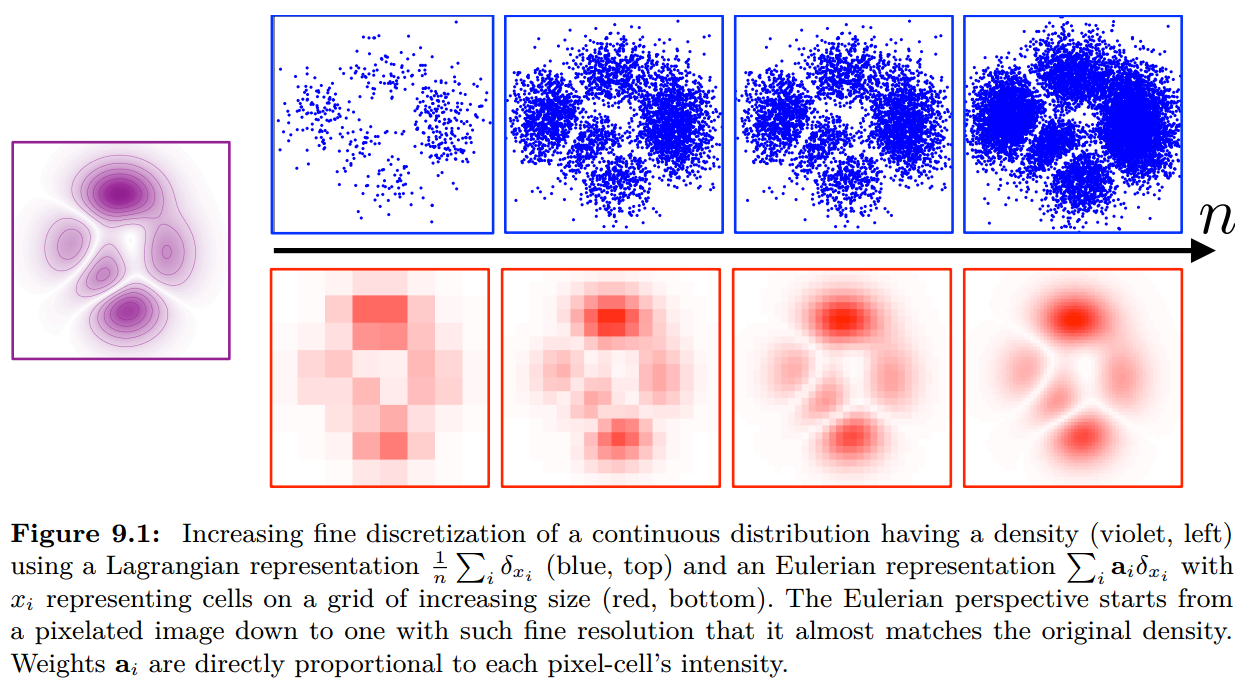
\includegraphics[scale = 0.3]{eulerian_lagrangian_comp.png}}
\end{minipage}
\caption{\footnotesize{\textbf{The comparison between Eulerian Discretization (down) and Lagrangian Discretization (top) \citep{gabriel2019computational} }}}
\label{fig: eulerian_lagrangian_comp}
\end{figure}
The optimal transport geometry has a unique ability, not shared with other information divergences, to leverage physical ideas (mass displacement) and geometry (a ground
cost between observations or bins) to compare measures. These two facts combined make it thus very tempting to use the Wasserstein distance as a loss function.  

However, the main technical challenge associated with that idea lies in approximating and \textbf{differentiating} efficiently the Wasserstein distance.  We start this section by presenting methods to approximate such gradients, then follow with three important applications that can be cast as variational Wasserstein problems.

We consider a \textbf{statisical estimation problem}: given a probability distribution $\beta$ arising from measurements, we need to find a model from a parameterized family of distributions $\{\alpha_{\theta}, \theta \in \Theta\}$ that \textbf{minimizes} the \emph{\textbf{Wasserstein distance}}, where $\Theta$ is a subset of a Euclidean space.
\begin{align}
\min_{\theta \in \Theta} & \cL_{c}(\alpha_{\theta}, \beta) \label{eqn: stats_estimation_ot}
\end{align} where $\cL_{c}(\alpha_{\theta}, \beta)$ is defined as the optimal value of \eqref{eqn: optimal_transport_prob}. This problem in general is \textbf{non-convex}. For cases such as Gaussian measures or elliptically contoured distributions, the \textbf{Wasserstein distance based objective} function has closed form, which can be solved directly. 

In most cases, however, one has to resort to a careful \textbf{discretization} of $\alpha_{\theta}$ to compute a \textbf{local minimizer} for Problem \eqref{eqn: stats_estimation_ot}. Two approaches can be envisioned: Eulerian or Lagrangian. Note that the discrete measure is $\alpha = \sum_{i}^{n}a_{i}\delta_{\mb{x}_{i}}$, which depends on two elements: the \textbf{position} of mass $\mb{X} := \{\mb{x}_{1}, \ldots, \mb{x}_{n}\}$ and the \textbf{probability measure} at each position $\mb{a}:= \{a_{1},\ldots, a_{n}\}$. Figure \ref{fig: eulerian_lagrangian_comp} compares the Eulerian discretization and Lagrangian discretization. 

\subsection{Eulerian and Lagrangian discretization}
\begin{itemize}
\item \textbf{Eulerian Discretization} (when the \underline{\textbf{measure}} of mass changes but the position of mass does not)\\
A first way to discretize the problem is to suppose that both distributions  $\alpha = \sum_{i=1}^{n}a_i \delta_{\mb{x}_{i}}$ and $\beta = \sum_{i=1}^{m}b_i\delta_{\mb{y}_{i}}$ are discrete distributions defined on fixed locations $\mb{X} = \{\mb{x}_{1}, \ldots, \mb{x}_{n}\}$ and $\mb{Y} = \{\mb{y}_{1}, \ldots, \mb{y}_{m}\}$.  The parameterized measure $\alpha_{\theta}$ is in that case entirely represented through the weight vector $a: \theta \rightarrow a(\theta) \in \Delta_n$, which, in practice, might be very sparse if the grid is large. This setting corresponds to the so-called class of \textbf{Eulerian discretization methods}.

In order to obtain differentiable objective function, we use the maximum entropy OT \eqref{eqn: optimal_transport_primal_entropy_reg}. The statistical estimation problem becomes
\begin{align}
\min_{\mb{\theta} \in \Theta} & L_{\mb{C}}^{\epsilon}(\mb{a}(\mb{\theta}), \mb{b}) := \cE_{E}(\mb{\theta}) \label{eqn: stats_estimation_max_ent_ot_eulerian}
\end{align} where $C_{i,j} = d(\mb{x}_{i}, \mb{y}_{j})$.

Recall that the maximum entropy OT objective is \textbf{differentiable} and \underline{\textbf{convex}} w.r.t. input historgrams, with gradient 
\begin{align}
\grad{(\mb{a}, \mb{b})}{L_{\mb{C}}^{\epsilon}(\mb{a}, \mb{b})} &= \brac{\begin{array}{c}
\mb{\lambda}_{*} \\
\mb{\mu}_{*}
\end{array}} \label{eqn: grad_max_ot_historgram}
\end{align} where $(\mb{\lambda}_{*}, \mb{\mu}_{*})$ are the \textbf{dual potentials} i.e. the optimal solutions of regularized dual problem \eqref{eqn: optimal_transport_dual_entropy_reg} chosen so that $\sum_{i}\lambda_i = \sum_{j}\mu_j = 0 $. The zero mean condition on $(\mb{\lambda}_{*}, \mb{\mu}_{*})$ is important when using gradient descent to guarantee conservation of mass. 

By chain rule, we have
\begin{align}
\grad{\mb{\theta}}{\cE_{E}(\mb{\theta})} = \grad{\mb{\theta}}{\mb{a}(\mb{\theta})}^{T}\mb{\lambda}_{*} \label{eqn: grad_loss_ruler}
\end{align} where $ \grad{\mb{\theta}}{\mb{a}(\mb{\theta})} \in \bR^{n \times d_{\theta}}$ is the Jacobian (differential) of the map $\mb{a}(\mb{\theta})$ and $d_{\theta} = \text{dim}(\mb{\theta})$.

The problem \eqref{eqn: stats_estimation_max_ent_ot_eulerian} is a convex optimization with differentiable gradient. It can be solved directly. 


\item \textbf{Lagrangian Discretization} (when the \underline{\textbf{position}} of mass changes)\\
A different approach consists in using instead fixed (typically uniform) weights and approximating an input measure $\alpha$ as an \textbf{empirical measure} $\alpha_{\mb{\theta}} =\frac{1}{n} \sum_{i=1}^{n}\delta_{\mb{x}_{i}({\mb{\theta}})}$ for a point-cloud parameterization map $\mb{X} : \mb{\theta} \rightarrow  \mb{X}(\mb{\theta}) = (\mb{x}(\mb{\theta})_i),$ where $\mb{x}(\mb{\theta})_i \in \cX$ for $i=1,\ldots, n$.  We assume here that $\cX$ is Euclidean. 

Note that the measure changes when the \textbf{position} of mass changes, which will affect the cost function $C_{i,j}$ as well. The optimization becomes
\begin{align}
\min_{\mb{\theta} \in \Theta} & L_{\mb{C}(\mb{\theta})}^{\epsilon}\paren{\frac{1}{n}\mb{1}_{n}, \mb{b}} := \cE_{L}(\mb{\theta}) \label{eqn: stats_estimation_max_ent_ot_lagrangian}
\end{align} where $\mb{C}(\mb{\theta}) := [c(\mb{x}_{i}({\mb{\theta}}), \mb{y}_{j})]_{i,j}$. Note that here the cost matrix $\mb{C}(\mb{\theta})$ now depends on $\mb{\theta}$ since the support of $\alpha_{\mb{\theta}}$ changes with $\mb{\theta}$. 

The objective function $L_{\mb{C}}^{\epsilon}(\mb{a}, \mb{b})$ can be represented as $L_{\mb{C}}^{\epsilon}(\mb{a}, \mb{b}) =\inn{\mb{P}^{*}}{\mb{C}} - \epsilon H(\mb{P}^{*})$. We can show that the function $g: \mb{C} \rightarrow g(\mb{C}) := L_{\mb{C}}^{\epsilon}(\mb{a}, \mb{b})$ is a  \underline{\textbf{concave}} and \textbf{smooth} function. The gradient of $g$ is
\begin{align}
\grad{\mb{C}}{L_{\mb{C}}^{\epsilon}(\mb{a}, \mb{b})} &= \mb{P}^{*} \label{eqn: grad_max_ot_cost}
\end{align} where $ \mb{P}^{*} = \diag{\mb{u}}\exp\paren{-\mb{C}/\epsilon}\diag{\mb{v}}$ is the optimal primal solution \eqref{eqn: optimal_transport_primal_entropy_reg} and it is also a function of $\mb{C}$.

By chain rule, we have
\begin{align}
\grad{\mb{\theta}}{\cE_{L}(\mb{\theta})} = \grad{\mb{\theta}}{\mb{X}(\mb{\theta})}^{T}(\grad{}{F(\mb{X}(\mb{\theta}))}) \label{eqn: grad_loss_lagrangian}
\end{align} where $\mb{X}(\mb{\theta}):= (\mb{x}(\mb{\theta})_i) \in \bR^{nd \times 1}$ and  $\grad{\mb{\theta}}{\mb{X}(\mb{\theta})} \in \bR^{nd \times  d_{\theta} }$ is the Jacobian matrix.
Here we define 
$F: \mb{X} \rightarrow L_{\mb{C}(\mb{X})}^{\epsilon}\paren{\frac{1}{n}\mb{1}_{n}, \mb{b}}$. Assuming $(\cX , \cY)$ are convex subsets of $\bR^d$, by chain rule we have 
\begin{align}
\grad{}{F(\mb{X})} &=\brac{\grad{\mb{C}}{L_{\mb{C}}^{\epsilon}(\mb{a}, \mb{b})}^T \grad{\mb{x}_{i}}{C}}_{i}\nonumber\\
&= \brac{\sum_{j}^{m}P_{i,j, *} \grad{\mb{x}_{i}}{c(\mb{x}_{i}, \mb{y}_{j})} }_{i=1}^{n} \in \cX^{n}  \label{eqn: grad_loss_cost}
\end{align} For instance, for $\cX = \cY = \bR^d$, for $c(s, t) = \norm{s - t}{2}^2$, one has 
\begin{align}
\grad{}{F(\mb{X})} &= 2\brac{\frac{1}{n}\mb{x}_{i} - \sum_{j}^{m}P_{i,j, *}\mb{y}_{j}}_{i=1}^{n} \in \cX^{n} \subset \bR^{nd}  \label{eqn: grad_loss_cost_eu}
\end{align} Note that, up to a constant, this gradient is $\text{Id} - T$ , where $T$ is the \textbf{barycentric projection}.
\end{itemize}

\subsection{Automatic differentiation}
Note that for both Eulerian and Lagrangian discretization, the gradient in \eqref{eqn: grad_loss_ruler} and \eqref{eqn: grad_loss_lagrangian} requires knowledge on the exact optimal solution $(\mb{\lambda}_{*}, \mb{\mu}_{*})$ on dual problem and  $\mb{P}^{*}$ on primal problem  This can only be achieved with acceptable precision using a very large number of \textbf{Sinkhorn iterates}. 

Given the limitation on time and computational resources, rather than approximating the gradient using the value obtained at a given iterate, it is usually better to \emph{differentiate} directly the \emph{output of Sinkhorn’s algorithm}, using \emph{\textbf{reverse mode automatic differentiation}}. In this case, we use the \textbf{\emph{Sinkhorn dual divergence}} $\mathfrak{D}_{\mb{C}}^{\epsilon}(\mb{a}, \mb{b}) :=\inn{\mb{\lambda}_{*}}{\mb{a}} + \inn{\mb{\mu}_{*}}{\mb{b}}$, which incorporates the entropy of the regularized optimal transport, and differentiating it directly as a composition of simple maps using the inputs, either the histogram in the Eulerian case or the cost matrix in the Lagrangian cases. 

Thus the objective for Eulerian and Lagrangian discretization becomes
\begin{align*}
(E):&\quad \mathfrak{D}_{\mb{C}}^{\epsilon}(\mb{a}(\mb{\theta}), \mb{b}) \\
(L):&\quad \mathfrak{D}_{\mb{C}(\mb{\theta})}^{\epsilon}\paren{\frac{1}{n}\mb{1}_{n}, \mb{b}}
\end{align*}

The cost for computing the \textbf{gradient} of functionals involving Sinkhorn dual divergences is \emph{the same as} that of computation of the \textbf{functional} itself.

\section{Wasserstein Barycenters and Clustering}
\subsection{Discrete measures}
Given input histogram $\{\mb{b}_s\}_{s=1}^{S}$, where $\mb{b}_s \in \Delta_{n_s}$, and weights $\mb{w} \in \Delta_{S}$, a Wasserstein barycenter is computed by minimizing
\begin{align}
\min_{\mb{a} \in \Delta_{n}}& \sum_{s=1}^{S}w_{s}L_{\mb{C}_{s}}(\mb{a}, \mb{b}_{s}) \label{eqn: ot_barycenter}
\end{align} where $\mb{C}_{s} \in \bR^{n \times n_s}$ is the cost matrix between $\mb{a}$ and $\mb{b}_{s}$. Typically, we assume $n_{s} = n$ and $\mb{C}_s = \mb{C} = \mb{D}^{p}, \forall s$ as distance matrix, and the problem becomes
\begin{align*}
\min_{\mb{a} \in \Delta_{n}}& \sum_{s=1}^{S}w_{s}\cW_{p}^{p}(\mb{a}, \mb{b}_{s})
\end{align*}

For discrete measures, this barycenter problem \eqref{eqn: ot_barycenter} is in fact a \emph{linear program}, since one can look for the $S$ couplings $(\mb{P}_s)_s$ between each input and the barycenter itself, which by construction must be constrained to share the same row marginal,
\begin{align*}
\min_{\substack{\mb{a} \in \Delta_{n},\\ \{\mb{P}_{s}\in \bR_{+}^{n\times n_s}, \forall s\}}}& \sum_{s=1}^{S}w_{s} \inn{\mb{P}_{s}}{\mb{C}_{s}} \\
\text{s.t. }& \mb{P}_{s}\mb{1}_{n_s} = \mb{a}, \forall s=1,\ldots, S\\
&\mb{P}_{s}^{T}\mb{1}_{n} = \mb{b}_{s}, \forall s=1,\ldots, S
\end{align*} This problem is a large-scale LP and can be solved using first order methods such as subgradient descent on the dual.

\subsection{Arbitrary measures}
Given input measuers $\{\beta_s\}_{s=1}^{S}$, where $\beta_s \in \cM_{+}(\cX)$, and weights $\mb{w} \in \Delta_{S}$, a Wasserstein barycenter for arbitrary measures is 
\begin{align}
\min_{\alpha \in \cM_{+}(\cX)}& \sum_{s=1}^{S}w_{s}\cL_{c}(\alpha, \beta_{s}) \label{eqn: ot_barycenter_cont}
\end{align} In the case where $\cX = \bR^d$ and $c(x, y) = \norm{x - y}{2}^2$, Agueh and Carlier show that if one of the input measures has a density, then this barycenter is \textbf{unique}. Moreover, under this condition, the \textbf{mean of the barycenter} $\alpha_{*}$ is necessarily the \textbf{barycenter of the mean}, i.e.
\begin{align}
\int_{\cX}x d \alpha_{*} &= \sum_{s=1}^{S}w_{s} \int_{\cX} x d\beta_{s}  \nonumber
\end{align} and the support of $\alpha_{*}$ is located in the \emph{convex hull} of the supports of the $\{\beta_s\}_{s=1}^{S}$.

Let us also note that it is possible to recast \eqref{eqn: ot_barycenter_cont} as a \textbf{multimarginal OT} problem.

\subsection{K-means as a Wasserstein variational problem}
When $\beta_s = \beta$ for all $s$ and $\cX = \bR^{d}$, $c(x, y) = \norm{x - y}{2}^2$, the barycenter problem becomes 
\begin{align*}
\min_{\alpha \in \cM_{k, 1}(\cX)}& \cL_{c}(\alpha, \beta)
\end{align*} where $\alpha = \sum_{i=1}^{k}a_i \delta_{\mb{c}_i}$ is constrained to be a \textbf{discrete measure} with a finite support of \textbf{size up to} $k$.  This barycenter problem  is equivalent to the usual \textbf{k-means} problem taking $\beta$. Indeed, one can easily show that the \textbf{\emph{centroids}} output $\{\mb{c}_{i}, i=1,\ldots, k\}$ by the k-means problem correspond to the \textbf{support} of the solution $\alpha$ and that its \emph{\textbf{weights}} $a_i$ correspond to the \textbf{fraction} of points in $\beta$ \emph{assigned to each centroid} \citep{canas2012learning}.

One can show that approximating $\cL \approx \cL^{\epsilon}$ using entropic regularization results in smoothed out assignments that appear in \textbf{soft-clustering} variants of k-means, such as \emph{mixtures of Gaussians}.

\subsection{Infinite mixtures and non-parametric Bayesian prior}
It is possible to generalize \eqref{eqn: ot_barycenter_cont} to a possibly \underline{\textbf{infinite collection of measures}}. This problem is described by considering a probability distribution $M$ over the space $\cM_{+}^{1}(\cX)$ of probability distributions, i.e. $M \in \cM_{+}^{1}(\cM_{+}^{1}(\cX))$. A \textbf{barycenter} is then a solution of
\begin{align}
\min_{\alpha \in \cM_{+}(\cX)}& \E{\beta \sim M}{\cL_{c}(\alpha, \beta)} :=  \int_{\cM_{+}^{1}(\cX)}\cL_{c}(\alpha, \beta)dM(\beta). \label{eqn: ot_barycenter_cont_infinity}
\end{align} where $\beta$ is a \emph{random measure} distributed according to $M$.  $M$ is a distribution over distributions, i.e. a \textbf{\emph{non-parametric Bayesian} prior}. Then we can see that the problem \eqref{eqn: ot_barycenter_cont} is a special case when $M = \sum_{s}w_s \delta_{\beta_{s}}$ is a discrete measure with finite support on space of measures. 

Drawing $S$ measures uniformly randomly would results in $\{\hat{\beta}_s\}_{s=1}^{S}$ with weight $w_{i} = \frac{1}{S}$. Define the unique solution of corresponding barycenter problem as $\hat{\beta}_{S} = \arg\min_{\alpha}\sum_{s=1}^{S}\cL_{c}(\alpha, \hat{\beta}_{s}) /S$. It is shown that the barycenters $\hat{\beta}_{S}$ has consistency, i.e.
\begin{align*}
\cL_{c}(\hat{\beta}_S, \alpha_{*} ) &\stackrel{S \rightarrow \infty}{\rightarrow} 0
\end{align*} where $\alpha_{*}$ is the optimal solution of infinite mixture barycenter problem \eqref{eqn: ot_barycenter_cont_infinity}. The convergence is in expectation or with high probability. This can be interpreted as a \textbf{law of large numbers} over the \textbf{Wasserstein space}. 

\subsection{Special cases}
\begin{figure}
\begin{minipage}[t]{1\linewidth}
  \centering
  \centerline{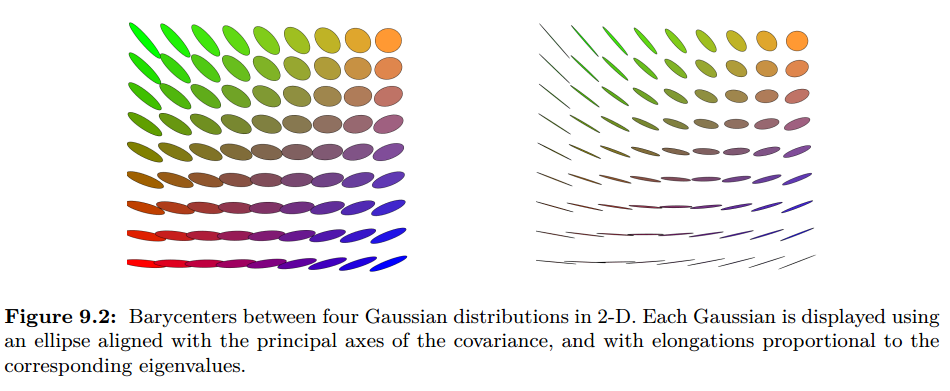
\includegraphics[scale = 0.45]{barycenter_gaussian.png}}
\end{minipage}
\caption{\footnotesize{\textbf{The smooth interpolation of Gaussian measures.}}}
\label{fig: barycenter_gaussian}
\end{figure}
\subsubsection{Barycenter of  Gaussian measures is Gaussian}
When all the measures are Gaussian $\beta_{s} = \cN(\mb{m}_{s}, \mb{\Sigma}_{s})$ for all $s$,  and $c(x, y) = \norm{x - y}{2}^2$,  the \textbf{barycenter} \eqref{eqn: ot_barycenter_cont} has a closed form solution and itself is a \textbf{Gaussian measure} $\alpha_{*} = \cN(\mb{m}_{*}, \mb{\Sigma}_{*} )$, where the \textbf{mean of barycenter} is the \textbf{barycenter of means} under Euclidean distance $c$
\begin{align}
\mb{m}_{*}&= \sum_{s=1}^{S}w_{s}\mb{m}_{s}  \nonumber
\end{align} and the \textbf{covariance} matrix of \textbf{barycenter} is the \textbf{barycenter of covariance matrices} under \textbf{\emph{Bures metric}}:
\begin{align*}
\mb{\Sigma}_{*}&= \arg\min_{\mb{\Sigma} \in \cS_{+}}\sum_{s=1}^{S}w_{s}\cB\paren{\mb{\Sigma}, \mb{\Sigma}_{s}}^2
\end{align*} This is a convex optimization problem and Bures metric is defined as 
\begin{align}
\cB\paren{\mb{\Sigma}_{\alpha}, \mb{\Sigma}_{\beta}}^2 &= \tr{\mb{\Sigma}_{\alpha} + \mb{\Sigma}_{\beta} - 2\paren{ \mb{\Sigma}_{\alpha}^{\frac{1}{2}}\mb{\Sigma}_{\beta}\mb{\Sigma}_{\alpha}^{\frac{1}{2}}}^{\frac{1}{2}}}.  \nonumber
\end{align}

$\mb{\Sigma}_{*}$ is the fix-point solution of the following map
\begin{align*}
\mb{\Sigma}_{*} &= \Phi(\mb{\Sigma}_{*}) \\
\text{where }\Phi(\mb{\Sigma}_{*})&=  \sum_{s=1}^{S}w_{s}\paren{ \mb{\Sigma}_{*}^{\frac{1}{2}}\mb{\Sigma}_{s}\mb{\Sigma}_{*}^{\frac{1}{2}}}^{\frac{1}{2}}
\end{align*}


\subsubsection{1-dimensional distributions on $\bR$}
For 1-D distributions, the $\cW_p$ barycenter can be computed almost in closed form using the fact that the transport is the monotone rearrangement. For empirical distribution $\beta_{s} := \frac{1}{n}\sum_{i=1}^{n}\delta_{y_{i,s}}$ , where the points are assumed to be \emph{\textbf{ordered}} $y_{1,s} \le y_{2,s} \le  \ldots  \le y_{n,s}$. The barycenter $\alpha_{w}$ is also an empirical measure on $n$ points
\begin{align*}
\alpha_{w} = \frac{1}{n}\sum_{i=1}^{n}\delta_{x_{i,w}}
\end{align*} where  the mass location $x_{i,w}$ is the result of barycenter map $ A_{w}$
\begin{align*}
x_{i,w} = A_{w}(y_{i,s}) := \arg\min_{x\in \bR}\sum_{s=1}^{S}w_{s}\norm{x - y_{i,s}}{p}^{p}; \quad \forall\, i=1,\ldots, S.
\end{align*} For instance, for $p = 2$, one has $x_{i,w} = \sum_{s=1}^{S}w_{s} y_{i,s}$ for all $i$. 

In the general case, one needs to use the cumulative functions. Recall that the inverse of c.d.f,  the generalized quantile function $F_{\alpha}^{-1}: [0,1] \rightarrow \bR\cup\set{-\infty}$ is defined as
\begin{align*}
F_{\alpha}^{-1}(r) &:= \min_{x}\set{x \in \bR\cup\set{-\infty}: \; F_{\alpha}(x) \ge r}. 
\end{align*} The $\cW_{p}$ distance is computed as 
\begin{align*}
\cW_{p}(\alpha, \beta)^{p} = \int_{0}^{1}\norm{F_{\alpha}^{-1}(r) - F_{\beta}^{-1}(r)}{p}^{p} dr 
\end{align*} So the \textbf{quantile} function of the \emph{barycenter} is computed via the barycenter map
\begin{align*}
F^{-1}_{\alpha}(r) &= A_{w}(F^{-1}_{\beta_{s}}(r))_{s=1}^{S} = \argmin_{g}\sum_{s}^{S}w_{s} \norm{g- F_{\beta_s}^{-1}}{L_p}^{p}
\end{align*} which can be used, for instance, to compute barycenters between discrete measures supported on less than n points in $O(n \log(n))$ operations, using a simple sorting procedure.

\subsubsection{Affine push-forward measures}
Consider that all $\beta_{s} = T_{r_s, u_s,\#}\alpha_{0}$ are push-forward measures from some base measure $\alpha_0$. The map $T_{r, u}: x \rightarrow r\,x + u$ is \textbf{affine}, i.e. via scaling and translation. It can be shown that the barycenter $\alpha_{*}$ of $\set{\beta_{s}}$ is a \textbf{push-forward measure} from  $\alpha_{0}$
\begin{align*}
\alpha_{*} = T_{r_{*}, u_{*},\#}\alpha_{0} &\\
\text{where } r_{*} = \paren{\sum_{s}w_s / r_{s} }^{-1}\;\; &\text{ i.e. the harmonic mean}\\
u_{*} = \sum_{s}w_{s} u_s  \;\;&\text{ i.e. the arithmetic mean}
\end{align*}

\subsection{Entropic approximation}
One can use entropic smoothing and approximate the solution of \eqref{eqn: ot_barycenter_cont} using
\begin{align}
\min_{\alpha \in \cM_{+}(\cX)}& \sum_{s=1}^{S}w_{s}\cL_{c}^{\epsilon}(\alpha, \beta_{s}) \label{eqn: ot_barycenter_ent_cont}
\end{align} for some $\epsilon >0$. This is a \textbf{smooth} \textbf{convex} minimization problem, which can be tackled using gradient descent. 
\subsubsection{Primal solution and generalized Sinkhorn algorithm}
The problem \eqref{eqn: ot_barycenter_ent_cont} can be reformulated using KL divergence
\begin{align}
 \min_{\mb{P}_s \in \bR_{+}^{n \times n_s}, \forall s}& \sum_{s=1}^{S}w_{s}\kl{\mb{P}_s}{\mb{K}_s}  \label{eqn: ot_barycenter_kl}\\
 \text{s.t. } &\mb{P}_s^{T}\mb{1}_{n} = \mb{b}_s, \quad s=1,\ldots, S\nonumber \\
 & \mb{P}_1\mb{1}_{n_1} = \ldots = \mb{P}_s\mb{1}_{n_s}\nonumber
\end{align}

The optimal solution is
\begin{align}
\mb{P}_s &=  \diag{\mb{u}_s}\mb{K}_{s}\diag{\mb{v}_s}, \quad s=1,\ldots, S  \label{eqn: ot_barycenter_kl_sol}
\end{align}
and the scalings are sequentially updated via \textbf{generalized Sinkhorn algorithm}
\begin{align}
\mb{v}_{s, t+1} &\leftarrow \frac{\mb{b}}{\mb{K}_{s}^{T}\mb{u}_{s, t}} :=\mb{b}\oslash \mb{K}^{T}\mb{u}_{s, t}   \label{eqn: ot_barycenter_sinkhorn_v}\\
\mb{u}_{s, t+1} &\leftarrow \frac{\mb{a}_{t+1}}{\mb{K}_{s}\mb{v}_{s, t+1}} := \mb{a}_{t+1}\oslash \mb{K}\mb{v}_{s, t+1} \label{eqn: ot_barycenter_sinkhorn_u} \\
\text{where } \mb{a}_{t+1}&= \prod_{s}^{S}\paren{\mb{K}\mb{v}_{s, t+1}}^{w_s} \; \text{ i.e. the geometric mean} \nonumber
\end{align}

\begin{figure}
\begin{minipage}[t]{1\linewidth}
  \centering
  \centerline{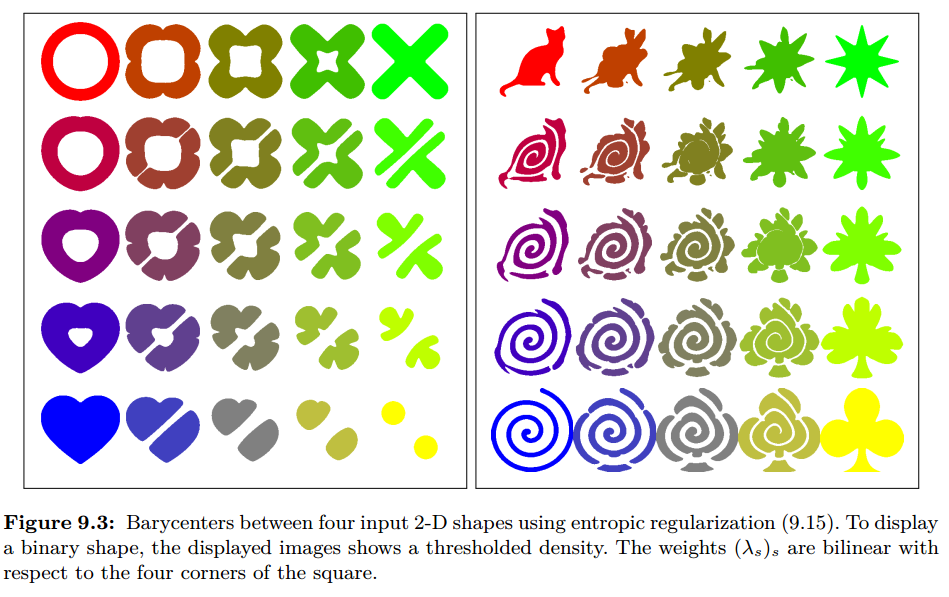
\includegraphics[scale = 0.4]{barycenter_ent_reg.png}}
\end{minipage}
\caption{\footnotesize{\textbf{The barycenter shape obtained via entropic regularization \citep{gabriel2019computational} }}}
\label{fig: barycenter_ent_reg}
\end{figure}

\subsubsection{Dual problem}
The optimal $(\mb{u}_{s, *}, \mb{v}_{s, *})$ appearing in \eqref{eqn: ot_barycenter_kl_sol} can be written as $(\mb{u}_{s, *}, \mb{v}_{s, *}) =
(\exp(\mb{\lambda}_{s, *}/\epsilon), \exp(\mb{\mu}_{s, *}/\epsilon))$, where $(\mb{\lambda}_{s, *}, \mb{\mu}_{s, *})$ are the solutions of the following dual program
\begin{align}
 \max_{(\mb{\lambda}_s , \mb{\mu}_s), \forall s}&  \sum_{s=1}^{S}w_s\set{\inn{\mb{\mu}_s}{\mb{b}_s} - \epsilon \inn{\exp\paren{\mb{\lambda}_s/\epsilon}}{\mb{K}_s\exp\paren{\mb{\mu}_s/\epsilon}}} \label{eqn: eqn: ot_barycenter_ent_dual} \\
 \text{s.t. }& \sum_{s=1}^{S} w_s \mb{\lambda}_s = \mb{0} \nonumber
\end{align} As with the original case, the generalized Sinkhorn algorithm  \eqref{eqn: ot_barycenter_sinkhorn_v} and \eqref{eqn: ot_barycenter_sinkhorn_u} can be obtained by alternating minimization with respect to  $\mb{\mu}_s$ and $\mb{\lambda}_s$. 


\subsection{Wasserstein propagation}
It is possible to generalize the barycenter problem \eqref{eqn: ot_barycenter}, where one looks for distributions $(\mb{b}_u)_{\cU}$ at some given set $\cU$ of nodes in a \underline{\textbf{graph}} $\cG = (\cU\cup\cV, \cE)$ given a set of fixed input distributions $(\mb{b}_v)_{\cV}$ on the \emph{complementary} set $\cV$ of the nodes.  The unknown are determined by minimizing the overall transportation distance between \textbf{all pairs of nodes} $(u, v) \in \cE$ forming edges in the graph
\begin{align*}
\min_{\{\mb{b}_{u} \in \Delta_{n_u}\}_{\cU}}&\sum_{(u, v) \in \cE} L_{\mb{C}_{u, v}}(\mb{b}_{u}, \mb{b}_{v}) 
\end{align*} where the cost matrices $\mb{C}_{u, v} \in \bR^{n_u \times n_v}$ need to be specified by the user.

The barycenter problem \eqref{eqn: ot_barycenter} is a special case of this problem where the considered graph $\cG = (\cU\cup\cV, \cE)$ is \underline{\textbf{star-shaped}}, where $\cU$ is a single vertex connected to all the other vertices $\cV$ (the weight $w_s$ associated to $\mb{b}_s$ can be absorbed in the cost matrix). Introducing explicitly a coupling $\mb{P}_{u,v} \in U(\mb{b}_u, \mb{b}_v)$ for each edge $(u, v) \in \cE$, and using entropy regularization, one can rewrite this problem similarly as in \eqref{eqn: ot_barycenter_kl}, and one extends Sinkhorn iterations \eqref{eqn: ot_barycenter_sinkhorn_v} and \eqref{eqn: ot_barycenter_sinkhorn_u}.


\section{Minimum Kantorovich Estimators}
\subsection{Challenges for Maximum Likelihood Estimation}
Given empirical measures $\beta_{n} = \sum_{i=1}^{n}\frac{1}{n}\delta_{\mb{x}_{i}}, \;\; \mb{x}_i \subset \cX$, i.i.d generated from some unknown distribution $\beta_{*}$, the goal of model estimation is to fit a parametric model $\theta \rightarrow  \alpha_{\theta} \in \cM(\cX)$ to the observed empirical input measure $\beta_{n}$. The standard \emph{\textbf{Maximum Likelihood Estimation (MLE)}} minimize the \emph{negative log-likelihood function} 
\begin{align*}
\min_{\theta}\;&\cL_{MLE}(\alpha_{\theta}, \beta_{n})
\end{align*} where $\alpha_{\theta}$ has density $\rho_{\theta}$ with respect to Lebesgue measure and $\cL_{MLE}(\alpha_{\theta}, \beta_{n}) = -\sum_i \log \rho_{\theta}(\mb{x}_i)$. We know that the MLE convergences to KL divergence $\cL_{MLE}(\alpha, \beta_{n}) \rightarrow \kl{\alpha}{\beta_{*}}$ where $\beta_{*}$ is the underlying distribution of data.

MLE has \textbf{challenges} to estimate $\alpha_{\theta}$ that is \emph{\textbf{singular}}, i.e. does not have density function $\rho_{\theta}$ w.r.t.  Lebesgue measure, or when the underlying distribution $\beta_{*}$ is \emph{\textbf{singular}}. In both cases, the KL divergence is not well defined since the support of $\alpha_{\theta}$ and $\beta$ may not overlap. Another issue is when $\rho_{\theta}$ is complicated and hard to compute. 

One typical case is when the task is to learn a genertive model $\alpha_{\theta}$ lies on a \emph{\textbf{low-dimensional}} \emph{\textbf{sub-manifold}}. Define the transform map $h_{\theta}: \cZ \rightarrow \cX$ so that 
\begin{align*}
\alpha_{\theta} = h_{\theta, \#}\zeta, \quad \zeta \in \cM(\cZ)
\end{align*} where $\cZ$ is a low-dimensional subspace.  Usually, $\alpha_{\theta}$ does not have density w.r.t. Lebesgue measure on $\cX$ since its support does not cover the entire space $\cX$. Furthermore, computing this density is usually intractable, while generating i.i.d. samples from $\alpha_{\theta}$ is achieved by computing $\mb{x}_i = h_{\theta}(\mb{z}_i)$, where $(\mb{z}_i)_i$ are i.i.d. samples from $\zeta$. 

For instance, in low-rank covariance esitmation, $\mb{x} = \mb{A}\mb{z}$, where $\mb{A} \in \bR^{d \times r}$, $\mb{z} \sim \cN(\mb{0}, \mb{\Sigma}_{z})$,  $\mb{\Sigma}_{x} = \mb{A}\mb{\Sigma}_{z}\mb{A}^{T}$ has rank $r \le d$. This is the degenerate case for covariance estimation.

\subsection{Learning generative models with Minimum Kantorovich Estimators}
We can use the Wasserstein distance as objective function in place of MLE objective. In particular, for Lipschitz function $f$ , we can write $\cW_1$ in its dual form as 
\begin{align}
\cW_1(\alpha, \beta) = \cL_{c}(\alpha, \beta) := \sup_{f \in \text{Lip}_1} \set{\int_{\cX} f(x) d\alpha_{\theta}(x)  - \int_{\cX} f(x) d\beta(x)} \label{eqn: wasserstein_1_dual}
\end{align} Note that since $\alpha_{\theta} = h_{\theta, \#}\zeta$, we have $f(x)d\alpha_{\theta}(x)  = f(x)d (h_{\theta, \#}\zeta)(x) = f(h_{\theta}(z)) d\zeta(z)$. The estimation problem becomes 
\begin{align}
\min_{\theta}\;&\cL_{c}(\alpha_{\theta}, \beta_{n}) = \cL_{c}(h_{\theta, \#}\zeta, \beta_{n})  \label{eqn: min_kantorovich_est}\\
\Rightarrow \min_{\theta}&\inf_{\pi \in U(\zeta, \beta_{n})}\E{\pi}{c(h_{\theta}(Z), Y )}     \quad\text{ (primal)} \label{eqn: min_kantorovich_est_primal}\\
\Rightarrow \min_{\theta}&\sup_{f \in  \text{Lip}_1}\set{\E{Z \sim \zeta}{f(h_{\theta}(Z))}  -  \E{X \sim \beta_{n}}{f(X)}}      \quad\text{ (dual)}\label{eqn: min_kantorovich_est_dual}
\end{align} The optimal transportation distances are weaker than MLE since  they are not invariant to important families of invariances, such as rescaling, translation or rotations. 

\begin{figure}
\begin{minipage}[t]{1\linewidth}
  \centering
  \centerline{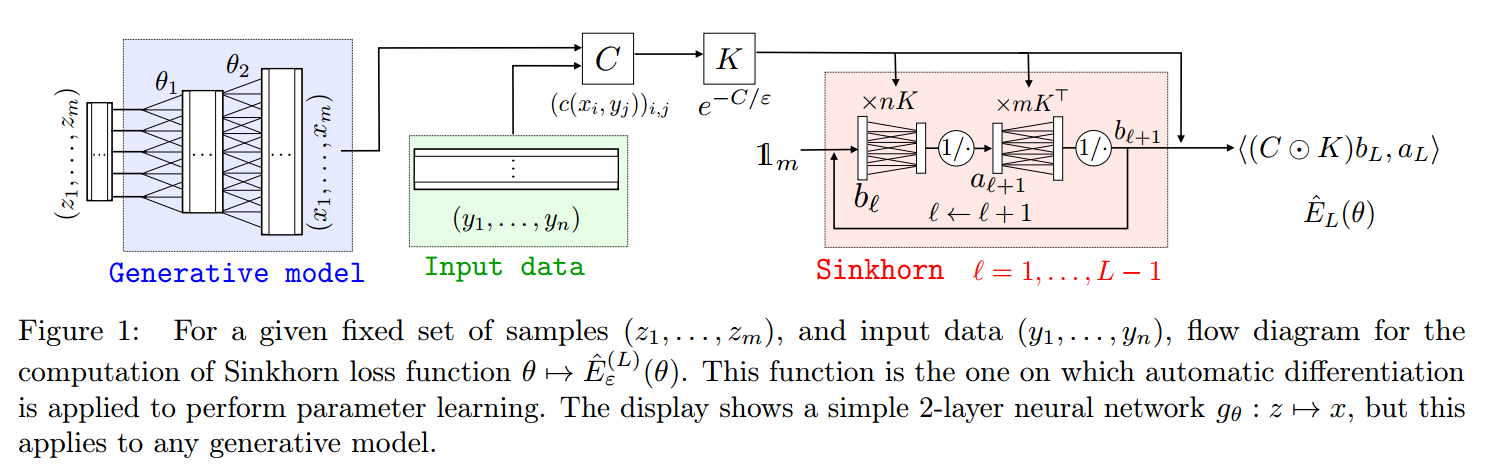
\includegraphics[scale = 0.3]{model_learning_sinkhorn_divergence.png}}
\end{minipage}
\caption{\footnotesize{\textbf{Learning generative model with Sinkhorn divergence \citep{genevay2018learning} }}}
\label{fig: barycenter_ent_reg}
\end{figure}


For $\cE(\theta):=\cL_{c}(\alpha_{\theta}, \beta_{n})$ , we can compute the subgradient function based on dual \eqref{eqn: wasserstein_1_dual} when the \textbf{dual potential} function $f$ is available, 
\begin{align}
\grad{\theta}{\cE(\theta)} &= \int_{\cZ} \brac{\grad{\theta}{h_{\theta}(z)}}^{T}\grad{}{f(h_{\theta}(z))} d\zeta(z)  \label{eqn: min_kantorovich_est_dual_grad}
\end{align} Here $\grad{}{f(x)}$ is gradient w.r.t. $x=h_{\theta}(z)$ and $\grad{\theta}{h_{\theta}(z)}$ is the differential (with respect to $\theta$) of $h_{\theta}$.

This formula is hard to use numerically, first because it requires first computing a continuous function $f$, which is a solution to a semi-discrete problem \eqref{eqn: optimal_transport_dual_prob}.  For OT loss, this can be achieved using stochastic optimization, but this is hardly applicable in high dimension. Another option is to impose a \emph{parametric} form for this \textbf{potential}, for instance expansion in an \emph{RKHS} or a \emph{\textbf{deep-network approximation}}. (e.g. the \underline{\textbf{\emph{Wasserstein GAN}}} \citep{arjovsky2017wasserstein}). A last issue is that it is \textbf{unstable} numerically because it requires the
computation of the gradient $\grad{}{f(x)}$ of the dual potential $f$.

We can also solve the primal problem directly, which is a semi-discrete problem. Note that $\beta_{n} = \sum_{i=1}^{n}\frac{1}{n}\delta_{\mb{x}_{i}}, \;\; \mb{x}_i \subset \cX$, thus the objective becomes
\begin{align}
\min_{\{\pi_i \in \cM_{+}(\cZ)\}_{i}^{n}, }\;&\sum_{i}^{n}\int_{\cZ}c(h_{\theta}(z), \mb{x}_i) d\pi_i(z)   \label{eqn: min_kantorovich_est_primal_semi}\\
 \text{where }& \sum_{i}d\pi_i(z) = \frac{1}{n} \nonumber \\
 &\sum_{i}\pi_i(z) = \zeta \nonumber
\end{align}
Based on \eqref{eqn: min_kantorovich_est_primal_semi}, we can obtain gradient
\begin{align}
\grad{\theta}{\cE(\theta)} &=  \sum_{i}^{n} \int_{\cZ} \brac{\grad{\theta}{h_{\theta}(z)}}^{T}\grad{1}{c(h_{\theta}(z), \mb{x}_i)}d\pi_i(z),  \label{eqn: min_kantorovich_est_primal_grad}
\end{align} where $\grad{1}{c(x,y))}$ is the gradient of $c$ w.r.t. first argument $x$. Note that as opposed to \eqref{eqn: min_kantorovich_est_dual_grad},
this formula does not involve computing the gradient of the potentials being solutions of the dual OT problem.

The class of estimators obtained using $\cL = \cL_c$, often called \textbf{minimum Kantorovich estimators}, was initially introduced in \citep{bassetti2006minimum}, also \citep{canas2012learning}; It has been used in the context of generative models by \citep{montavon2016wasserstein} to train restricted Boltzmann machines and in \citep{bernton2017inference} in conjunction with approximate Bayesian computations. Approximations of these computations using Deep Network are used to train deep generative models for both \textbf{\emph{GAN}} \citep{arjovsky2017wasserstein} and \textbf{\emph{Variational Auto-Encoder (VAE)}} \citep{tolstikhin2018wasserstein}; see also \citep{genevay2017gan, genevay2018learning, salimans2018improving}. Note that the use of \textbf{Sinkhorn divergences} for parametric model fitting is used routinely for \textbf{shape matching} and \textbf{registration}, see \citep{gold1998new, rangarajan2000applications, myronenko2010point, feydy2017optimal}.

OT can also be applied to \textbf{metric learning} to learn cost function $c$ \citep{wang2012supervised, cuturi2014ground, zen2014simultaneous, huang2016supervised}; or to \textbf{domain adaptation} \citep{flamary2016optimal} and transfer learning \citep{pan2009survey}.

\newpage
\bibliographystyle{plainnat}
\bibliography{book_reference.bib}
\end{document}